\documentclass[12pt,a4paper]{amsart}
\usepackage[T1]{fontenc}
\usepackage[british]{babel}
\usepackage{lmodern,microtype}
\usepackage[margin=28.8mm]{geometry}
\usepackage{amsmath,amssymb,mathtools}
\usepackage{tikz}
\usepackage[numbers]{natbib}
\usepackage{xurl}
\usepackage[colorlinks=true,linkcolor=blue!45!black,citecolor=blue!45!black,urlcolor=blue!45!black]{hyperref}
\newtheorem{proposition}{Proposition}
\newcommand{\E}{\mathbb E}
\newcommand{\Var}{\operatorname{Var}}
\newcommand{\Prb}{\mathbb P}
\raggedbottom

\title[Measuring human labour]{Measuring human labour in AI-assisted software engineering}
\date{}
\keywords{software engineering, labour measurement, partial identification, probability sampling, AI assistance}
\hypersetup{pdftitle={Measuring human labour in AI-assisted software engineering}}
\begin{document}

\begin{abstract}
Teams can produce the same sequence of commits after spending different amounts of time on a requirement. We bound labour in a chosen period using observations of hours worked and the time each contributor had available. When contributors can switch freely among the permitted activities within each interval, every total between the bounds fits the observations. If a task must run continuously, a break in the contributor’s availability can exclude intermediate totals that would be possible if the task could be split. Across 96 possible patterns of work in a two-person shift, limiting the engineer's combined task hours to the time available reduced the mean width of the first-hour labour range from 1.5 to 0.5 person-hours. Omitting the reviewer excluded the actual total in 26 cases. To estimate full-shift labour, we sampled two of four one-hour intervals and doubled the hours worked in the selected intervals. The mean sampling variance across shift patterns was $49/72$ squared person-hours. Using those hours to correct a predicted shift total reduced it to $25/72$. For simple random sampling, we derive a conservative confidence interval for total labour that allows for hours left unknown after follow-up. A hypothetical trial illustrates how omitted review hours and failed checks counted as passes can produce a false claim of benefit from AI.
\end{abstract}
\maketitle

\section{What commit sequences reveal about working hours}
\label{sec:intro}

Suppose a team adds a month filter to its customer order export. It tests the filter with two orders dated 31 March and 1 April. Only the first belongs in the March export. An engineer spends one hour on the filter during a two-hour shift. The team wants to know how much of that work preceded a release halfway through the shift. The whole hour fits on either side, so the shift total alone allows anything from zero to 60 minutes before release.

With only commit times as evidence, even the shift total is uncertain. Suppose the engineer works on the filter in a given minute with probability $p$. A working minute produces a commit with probability $c$, and an idle minute produces none. What happens in one minute is independent of activity and commits in every other minute. The pairs $(p,c)=(1/2,1/5)$ and $(1/4,2/5)$ both give a commit probability of $1/10$ per minute. Every finite commit sequence therefore has the same probability under both models, although the expected time worked in an hour is 30 minutes in the first model and 15 in the second.

Wright and Ziegler used commit times to infer coding activity, then trained a predictor on the resulting labels \cite{wright2019}. Agreement with those labels leaves open how many hours people worked. A release discussion can occupy several engineers without producing a commit. An unattended AI workflow can produce one. Perry et al.\ compared developers' accounts of their time with direct observation \cite{perry1994}. Such observations can place work within a shift even when its exact timing remains unknown.

Peng et al.\ timed participants who finished a programming exercise \cite{peng2023}. Measuring labour would also require the time spent by participants who stopped before finishing. Cui et al.\ counted completed pull requests per week \cite{cui2026}. Splitting a change across several pull requests raises the count even if the team delivers the same functionality.

We use each person's shift total to bound the hours that could fall before a release. For a random sample of intervals, weighting the measured hours by the inverse of their selection probabilities estimates total labour. Both calculations start by specifying whose work counts and which requirements it serves.

\section{What the comparison must count}
\label{sec:accounting}

A requirement specifies how the software should behave. A task is the unit whose entry, first acceptance and labour the team tracks. In this comparison each task corresponds to one original requirement. The task enters when it meets the inclusion rules and its requirement has acceptance criteria. Give the requirement for task $i$ a fixed initial weight $s_i\ge 0$ at entry. For the export, the date filter carries two units, one for each date check. Preserving the leading zeros in order numbers is a second requirement worth one unit. The same scoring and acceptance rules apply in both groups.

An activity is something a contributor does on a task, such as implementing the date filter or reviewing its checks. We use \emph{work} as a general term for such effort and measure \emph{labour} in person-hours. Specify whose time counts and which kinds of activity qualify under the same rule for both groups. An activity is eligible for a task's labour total when a contributor in that population performs an included kind of work to deliver, check or repair the task's required behaviour during its labour window. When the target covers only part of the window, count only the overlap. Include external reviewers when the target is everyone's labour. Half an hour reviewing the date filter counts towards the filter task even if it leaves no commit. An unrelated support call during the same shift falls outside both export tasks. If a meeting serves several tasks, divide each participant's time among them so that an hour of attendance contributes at most one person-hour per participant.

Task age is elapsed time since entry, including time spent waiting. Choose a cutoff age $\tau\ge 0$ for first acceptance and a follow-up delay $\Delta\ge 0$ in the same time units. Let $T_i$ be the age at first acceptance, taking $T_i=\infty$ for a task never accepted. If $T_i\le\tau$, assess the fraction $R_i\in[0,1]$ of the requirement still satisfied at age $T_i+\Delta$. Its retained score is $Q_i=s_iR_i$. An accepted requirement with no follow-up assessment has an unknown retained score. A task still awaiting first acceptance at the cutoff contributes zero to that score. Score the original requirement once across retries and pull requests. For the date filter, rerun the March query at follow-up. Each date check still passing contributes one unit.

A task's labour window extends from entry through age $\tau+\Delta$. Count its person-hours $H_i$ throughout that window, including repairs after an early follow-up and work on tasks still awaiting acceptance. Summing over the included tasks gives the retained score $Q=\sum_i Q_i$ and labour $H=\sum_i H_i$. Their ratio $Q/H$ gives retained score per person-hour when $H>0$. For zero labour, give both totals. A proposed rate $\rho$ implies $Q=\rho H$. For positive labour, keep each $\rho$ for which a confidence interval for $Q-\rho H$ includes zero, accounting for how the two totals were sampled \cite{vonluxburg2009}.

For the paired trial in Section~\ref{sec:workplace}, divide each team's totals by its initial score $S=\sum_i s_i>0$. A team taking the two export tasks starts with $S=3$. Its hours per initial unit are $H/S$ and the fraction of its initial score retained is $Q/S$. If the team drops a task, its requirement's initial weight still counts in $S$ and the hours already worked count in $H$.

\section{Bounds from partial observations}
\label{sec:bounds}

A shift total can bound the hours worked before a release even when the start time is unknown. If one person spent $v$ hours on a task across two periods lasting $b$ and $c$ hours, the amount $x$ in the first period satisfies
\[
  \max(0,v-c)\le x\le\min(v,b).
\]
Any hours that exceed the capacity of the second period must fall in the first. The upper limit is the smaller of the task total and the duration of that first period.

Suppose an engineer spent one hour implementing a feature and one hour repairing a defect within a two-hour shift. Each activity can fill the first hour in a different schedule, as Figure~\ref{fig:shared-time} shows. Adding their separate maxima would assign two person-hours to an engineer with one hour available. The second hour can absorb at most one person-hour of the two-hour total. Exactly one person-hour therefore falls in the first hour.

\begin{figure}[ht]
\centering
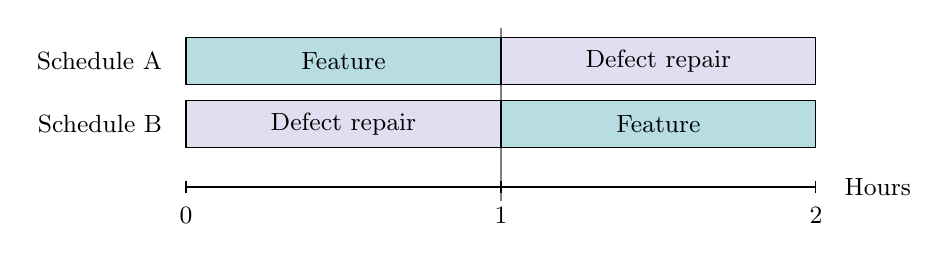
\begin{tikzpicture}[x=4.0cm,y=.8cm,font=\small]
  \definecolor{feature}{HTML}{B7DDE3}
  \definecolor{repair}{HTML}{E1DEF1}
  \draw[gray] (1,.15) -- (1,2.9);
  \draw[fill=feature] (0,2) rectangle (1,2.75);
  \draw[fill=repair] (1,2) rectangle (2,2.75);
  \draw[fill=repair] (0,1) rectangle (1,1.75);
  \draw[fill=feature] (1,1) rectangle (2,1.75);
  \node[anchor=east] at (-.045,2.375) {Schedule A};
  \node[anchor=east] at (-.045,1.375) {Schedule B};
  \node at (.5,2.375) {Feature};
  \node at (1.5,2.375) {Defect repair};
  \node at (.5,1.375) {Defect repair};
  \node at (1.5,1.375) {Feature};
  \draw (0,.38) -- (2,.38);
  \foreach \x in {0,1,2} {
    \draw (\x,.28) -- (\x,.48);
    \node[below=1.5pt] at (\x,.28) {\x};
  }
  \node[anchor=west] at (2.06,.38) {Hours};
\end{tikzpicture}
\caption{Two schedules consistent with one hour of feature work and one hour of repair by the same engineer. The first hour contains one person-hour in either schedule.}
\label{fig:shared-time}
\end{figure}


\subsection{Compute the range on a shared time axis}

Use $g$ to denote one contributor's activity on one task and $j(g)$ for that contributor. Cover the full span of each observation, including work outside the target when it shares an observed total with work in scope. Partition the time axis at every observation boundary and every target boundary. Each resulting cell $J_k$ has duration $d_k>0$ in hours. Let $x_{gk}$ be the person-hours of activity $g$ in cell $k$.

An observation $\nu$ supplies a range $[v^-_\nu,v^+_\nu]$ for the combined hours of activities $G_\nu$ during a set $K_\nu$ of whole cells. An exact measurement sets both endpoints equal. Widen the interval to allow for rounding or other known error. The arrays $x$ must satisfy
\begin{align}
 x_{gk} &\ge 0, &
 \sum_{g:j(g)=j}x_{gk} &\le d_k,\\
 v^-_\nu &\le \sum_{g\in G_\nu}\sum_{k\in K_\nu}x_{gk}
 \le v^+_\nu.
\end{align}
Nonnegativity holds for each activity in each cell. Apply the capacity limit to each contributor in each cell and the observation limit to every $\nu$. To represent an absence, cut at its boundaries and set that contributor's hours to zero in the affected cells.

Write $\mathcal P$ for the set of arrays satisfying the constraints. Sum the target hours as $h(x)=\sum_{g,k}w_{gk}x_{gk}$, with $w_{gk}=1$ for work in scope and $0$ elsewhere. If $\mathcal P$ is nonempty, solve two linear programmes to obtain
\begin{equation}
  [L,U]=\left[\min_{x\in\mathcal P}h(x),\,
                    \max_{x\in\mathcal P}h(x)\right].
  \label{eq:labour-bounds}
\end{equation}
Integrating any allocation that satisfies the observation and time limits yields an array in $\mathcal P$. The corresponding total therefore lies in $[L,U]$. An empty $\mathcal P$ means that the supplied limits are inconsistent under the accounting rules.

\subsection{When the endpoints can occur}

The cell model recovers exactly the possible totals when people can divide their time among eligible activities within each cell. One allocation uses a constant share $x_{gk}/d_k$ for every activity in that cell. If each person must work on one activity at a time, schedule each activity in one block of length $x_{gk}$ and leave any remaining time idle. One block per activity per cell suffices to recover the observations and the target total. The feasible set is closed and bounded, so both extrema exist. A weighted average of the two optimising arrays preserves all constraints and realises the corresponding intermediate total. The allocation argument applies to that array as well.

A minimum session length or fixed activity order can rule out some of these allocations. Equation~\eqref{eq:labour-bounds} still encloses every total that satisfies the added scheduling rules. The endpoints are tight if each occurs under those rules. Suppose an uninterrupted one-hour session must fit into one of two one-hour periods separated by an absence. The session contributes a full hour to whichever period contains it, so the first-period total can be zero or one hour.

A rule requiring two people to review together can enter the linear programme directly. Suppose a finite set of working configurations describes the combinations allowed at each instant. A configuration specifies each person’s activity or idle time. For paired review, the permitted configurations put both named reviewers on the review whenever either is reviewing. Allocate a nonnegative duration to each permitted configuration. Require their durations to sum to $d_k$. Then $x_{gk}$ is the sum of durations for configurations containing $g$. Each permissible allocation supplies the duration spent in each configuration. If the team can switch configurations within the cell, consecutive blocks of those lengths recover the observed totals.

\subsection{When the observations leave work uncovered}

If $[L,U]$ covers the included contributors' hours and an independent check caps uncounted hours at $B$, the combined total lies in $[L,U+B]$. When the extra hours have no established upper limit, restrict the conclusion to $[L,U]$ for the included contributors. For observations from a sample, the target range covers the true total whenever all observation ranges cover their respective values and the true allocation satisfies the capacity constraints. By the union bound, observation ranges with failure probabilities summing to at most $\alpha$ give target coverage of at least $1-\alpha$ even when the observations depend on one another.

\section{Estimating labour from a sample}
\label{sec:sampling}

Divide each contributor's observation period into disjoint intervals. Index the
eligible person-intervals by $U=\{1,\ldots,M\}$. Interval $m$ lasts $d_m$ hours
and contains $y_m\in[0,d_m]$ person-hours of work on the requirements. The target
is $H=\sum_{m\in U}y_m$. Select a sample $s$ with known inclusion probability
$\pi_m>0$ for every interval. Draw after the work period if asking during it could interrupt the activity. Inference holds the completed work history fixed and
averages over possible draws.

\subsection{Use predictions to reduce sampling variation}

Fix a prediction $f_m\in[0,d_m]$ for each interval before the draw and write
$r_m=y_m-f_m$ and $F=\sum_{m\in U}f_m$. If the selected hours are known, estimate
the total by
\begin{equation}
  \widehat H=F+\sum_{m\in s}\frac{r_m}{\pi_m}.
  \label{eq:short-difference}
\end{equation}
The indicator that interval $m$ is selected has expectation $\pi_m$. Thus the
expected weighted correction is $\sum_{m\in U}r_m$, and
$\mathbb{E}[\widehat H]=H$. Selections may depend on one another. Predictions
may have systematic errors because the correction estimates their total error.
Setting each $f_m$ to zero yields the Horvitz--Thompson estimator \cite{horvitz1952}.
The generalised difference estimator can reduce variation across draws
when predictions leave a less variable correction \cite{cassel1976}.

For a simple random sample drawn without replacement, suppose
$1\le n\le M$ and $M>1$. Then the variance of \eqref{eq:short-difference} is
$K_n S_r^2$, where $K_n=M^2(1-n/M)/n$ and $S_r^2$ is the population variance of
the residuals with divisor $M-1$. This follows from $\pi_m=n/M$ and the
finite-population variance of the sample mean. The direct estimator has
variance $K_n S_y^2$, with the hours themselves in place of the residuals.
For $n<M$, prediction correction improves precision exactly when
$S_r^2<S_y^2$. A census has zero sampling variance.

\subsection{Follow up missed observations or bound their effect}

Let $A$ be the intervals with usable initial answers. Randomly select $B$
from $s\setminus A$ so that each missed interval has known conditional
selection probability $\eta_m>0$. If both stages supply accurate hours for the
intervals they cover, the estimate is
\[
  F+\sum_{m\in A}\frac{r_m}{\pi_m}
   +\sum_{m\in B}\frac{r_m}{\pi_m\eta_m}.
\]
Conditional on $s$ and $A$, the second draw recovers the complete-sample
correction in \eqref{eq:short-difference} in expectation. Taking the expectation
over the first draw recovers $H$.
Workload may affect the initial answer rate \cite{nonresponsefollowup}.

When accurate hours remain unavailable, bound each selected interval by $[l_m,u_m]$ from the available observations. For a missed answer, the
physical limits $[0,d_m]$ suffice. The weighted estimate increases with each $y_m$. Evaluating it at the lower
limits yields $\widehat H^-$ and at the upper limits yields $\widehat H^+$.
The estimate that would have used the true sampled hours lies between these
values whenever every supplied range contains its true hours. These bounds
account for incomplete measurement on the selected intervals.

For simple random sampling, add a finite-sample margin for the draw itself.
All residuals lie between $a=-\max_{m\in U} f_m$ and
$b=\max_{m\in U}(d_m-f_m)$. The sum of squared deviations from their mean
is at most the sum of squared deviations from $(a+b)/2$, so
$S_r^2\le M(b-a)^2/[4(M-1)]$. Chebyshev's inequality gives a margin
\[
  e=\sqrt{\frac{K_n M(b-a)^2}{4(M-1)\alpha}}\qquad (0<\alpha<1).
\]
The interval $[\widehat H^--e,\widehat H^++e]$, intersected with the physical range
$[\sum_{m\in s}l_m,\;\sum_{m\in s}u_m+\sum_{m\notin s}d_m]$, covers $H$ with probability at least $1-\alpha$ when the
measurement limits hold on every draw. Use $e=0$ for a census, including
$M=1$. If the chance that any sample range excludes its true value is
at most $\beta$, coverage is at least $1-\alpha-\beta$ by the union
bound. The margin can be wide when little is known. If eligible work
outside the list has a defensible total capacity $D$, adding $D$ to the upper
limit covers the expanded target at the same level. A separate estimate
requires evidence about the time those contributors spent on the requirements.

\section{Checks against 96 known work histories}
\label{sec:results}

During a two-hour shift, one engineer implements a feature in two half-hour slots. Repair work occupies up to two of the remaining slots, and a colleague reviews the feature in one slot. Combining the 24 engineer schedules with four possible review slots produces 96 equally weighted histories. We count the occupied slots to establish the actual person-hours.

First ask whether the two contributors spent more than one person-hour in the first hour. The calculation receives the engineer's shift total for each task and the review totals for the first hour and full shift. We compare a separate capacity limit for each activity with one limit shared by the engineer's implementation and repair. A lower bound above one confirms excess labour. An upper bound of one or less rules it out. A range that permits both outcomes leaves the decision open.

\begin{table}[htbp]
\centering\small
\caption{Decisions about first-hour labour above one person-hour. Width is the mean range width in person-hours. Contains actual total counts the ranges that include both contributors' known labour.}
\label{tab:short-known-hours}
\begin{tabular}{@{}p{.38\linewidth}rrrrr@{}}
\hline
\shortstack[l]{Observations and capacity limit} & Width & \shortstack{Contains\\actual total} & Correct & Wrong & Open \\
\hline
Separate limits per activity & 1.5 & 96 & 12 & 0 & 84 \\
Shared limit across the engineer's tasks & 0.5 & 96 & 60 & 0 & 36 \\
Engineer's first-hour total also known & 0 & 96 & 96 & 0 & 0 \\
Reviewer omitted, shared limit & 0.5 & 70 & 70 & 26 & 0 \\
Review timing unknown, shared limit & 1.0 & 96 & 0 & 0 & 96 \\
\hline
\end{tabular}
\end{table}

The shared limit rules out overlapping uses of the engineer's time. Table~\ref{tab:short-known-hours} shows that it narrowed the mean range from 1.5 to 0.5 person-hours and increased the number of correct decisions from 12 to 60. Omitting the reviewer gave the same mean width of 0.5 person-hours and excluded the actual total in 26 histories. Entering zero for first-hour review time reproduces those errors. When the timing of the known half-hour of review is unknown, allow it to contribute anywhere from zero to half a person-hour in the first hour. For an engineer with $v\in[1,2]$ person-hours over the shift, the resulting range is $[v-1,1.5]$. This contains the actual total in every history and leaves every decision open.

Next estimate labour over the full shift. Each contributor has two one-hour intervals. We enumerate all six equally likely samples of two intervals per history, fixing predictions at 0.75 person-hours per engineer interval and 0.25 per reviewer interval. With accurate replies, both estimators average to the actual total within each history. Averaged across histories, the sampling variance is $49/72$ squared person-hours for direct weighting and $25/72$ with the prediction correction. If the reviewer supplies zero hours whenever sampled, both estimates fall short by half a person-hour on average. If the reviewer omits the reply covering the review, the complete-response procedure returns an estimate for only 288 of 576 draws.

These results describe the schedules and measurement failures specified in the check. A workplace audit must establish which contributors and intervals its inputs cover before the width of a range or the spread of estimates can support a decision.

\section{Checking an apparent saving}
\label{sec:workplace}

Before randomisation, each team fixes its set of tasks and scores their requirements. Suppose a team takes the two export tasks and both pass their acceptance checks by the cutoff. At follow-up the March export contains both orders. Including the April order costs the filter one unit. The repaired export still prints order number 007 with both leading zeros, so the repair retains its unit. The team retains two of its three initial units ($Q/S=2/3$). Its labour per unit includes all hours on those requirements through age $\tau+\Delta$, including work after the illustrated shift.

An independent fair draw in each matched pair selects the team offered the specified AI tools. For hours per initial unit and for the retained fraction, subtract the comparison team's value from the value for the team offered AI. If each team's outcomes depend only on its own offer, averaging these differences over pairs and possible draws gives the mean effect of the offer on the enrolled teams. A shared reviewer or code passed between teams can let one team's offer affect another team's outcome \cite{hudgens2008}.

The complete-data rule requires both outcomes from every team. To declare a benefit, the trial must establish a saving above one person-hour per initial unit with a retention loss below five percentage points. The teams must justify these thresholds before the trial \cite{piaggio2012}. In a separate example with six hypothetical pairs, counting every hour of work and scoring each check by whether it passed puts the mean saving and retention loss exactly at those thresholds. A benefit requires a larger saving and a smaller loss. Omitting one review hour per initial unit from the AI teams' accounts doubles their apparent saving. Each requirement has 100 equally weighted checks. Counting six failures as passes on each AI-team requirement turns a five-point loss into an apparent one-point gain. Together the errors produce a false benefit claim.

To check for omitted hours, select shifts independently of whether contributors replied. Compare their accounts with separate evidence of who worked on the requirements and for how long, including external review within the labour window. Allow for work absent from both sources by bounding how long each contributor could have spent on the requirements during the shift. On these shifts, compare the time contributors spend answering requests about sampled intervals with the time they spend giving a full daily account. Use the independent evidence to check omissions in each method. At follow-up, have independent reviewers retest the acceptance criteria and resolve discrepancies where the evidence permits.

Set the rules for bounding unobserved outcomes before the trial begins. Denote the number of enrolled pairs by $P\ge 1$ and index them by $h$. Calculate a separate difference $D_{ho}$ in each pair for each outcome $o$. Use $o=\mathrm{lab}$ for hours per initial unit and $o=\mathrm{ret}$ for the retained fraction. Before the draw, specify a finite range $[a_{ho},b_{ho}]$ that contains the difference whichever team receives the offer. After the draw, use the available measurements to bound the difference under the allocation actually drawn by $[\ell_{ho},u_{ho}]$. Use the range fixed before the draw if both teams lack that outcome.

Across pairs, the mean difference under the draw is $\overline D_o=P^{-1}\sum_{h=1}^{P}D_{ho}$. Write $\mu_o=\E[\overline D_o]$ for its expectation over possible draws. Fix the teams' potential outcomes under either offer. If outcomes in a pair depend only on that pair's draw, the independent draws make the pair differences independent. Hoeffding's inequality bounds the chance that $\overline D_o$ falls more than $\varepsilon_o$ below $\mu_o$ by $\alpha_o$. The same bound holds above $\mu_o$ \cite{hoeffding1963}. For $0<\alpha_o<1$, the margin is
\[
\varepsilon_o=\sqrt{\frac{\log(1/\alpha_o)}{2P^2}
  \sum_{h=1}^{P}(b_{ho}-a_{ho})^2}.
\]
Let $\overline{\ell}_o$ and $\overline{u}_o$ be the averages of the lower and upper limits across pairs after the draw. If each range contains its pair's difference, then $\overline{\ell}_o\le\overline D_o\le\overline{u}_o$. A benefit requires the upper confidence limit for labour, $\overline{u}_{\rm lab}+\varepsilon_{\rm lab}$, to fall below $-1$ person-hour per initial unit. The lower confidence limit for retention, $\overline{\ell}_{\rm ret}-\varepsilon_{\rm ret}$, must exceed $-0.05$.

For outcome $o$, suppose the chance that any pair's range excludes its actual difference is at most $\gamma_o\in[0,1]$. A confidence limit can exclude $\mu_o$ only if a pair's range excludes its difference or the draw takes the mean beyond the corresponding one-sided margin. By the union bound the chance is at most $\alpha_o+\gamma_o$. If a true effect fails its threshold, a false benefit claim requires the confidence limit for that outcome to fail. The larger of the two error bounds therefore covers the chance of a false claim whichever threshold fails.

For 48 pairs with labour differences between $-10$ and $10$ person-hours per initial unit, $\alpha_{\rm lab}=0.025$ gives a margin of about 3.92 in those units. Even with exact measurements, the observed mean saving would have to exceed about 4.92 person-hours per initial unit to establish a saving above one. On the preliminary shifts, check which contributors could have worked on each requirement and how many hours each had available. Use those hours and each team's initial score to justify the range of possible differences in labour per initial unit. Before the main trial, simulate the rule across effects that meet or fail its thresholds to estimate how often it detects a benefit or declares one in error.


\section{Conclusion}

Omitting the export review reduces the counted work before release from 1.5 person-hours to one. Across all 96 shift patterns, the mean range width gave no indication of the omission. To investigate an apparent saving, trace a change through review and repair. Where a contributor's hours are uncertain, calculate the saving across the range of hours the evidence permits. The labour saving supports a benefit claim only if the follow-up check also shows that enough of the original functionality still works.

\section*{Data and code availability}

The \href{https://github.com/emmett08/engineering-work-observatory/tree/4847fee965041b1a6ac7cf26b317a9c9c9181722/paper}{full paper and reproducibility materials} contain the 96 enumerated shift patterns and the trial examples. The repository includes the source and model notes for this shorter paper.

\bibliographystyle{plainnat}
\bibliography{references}
\end{document}
